\documentclass[sigconf]{acmart}

\usepackage[utf8]{inputenc}

\usepackage{booktabs} % For formal tables
\usepackage{graphicx}
\usepackage{rotating}
\definecolor{Gray}{gray}{0.6}
\usepackage{tabularx}
\usepackage{xspace}
\usepackage{float}
\usepackage{xstring} % for string operations
\usepackage{wasysym} % Table legend with symbols input from post-processing
\usepackage{MnSymbol} % Table legend with symbols input from post-processing
\usepackage{ifthen}

\usepackage{diagbox}
\usepackage{url}
\usepackage{multirow}% http://ctan.org/pkg/multirow

\settopmatter{printacmref=false}
\usepackage{amsmath}
\usepackage{algorithm}% http://ctan.org/pkg/algorithms
\usepackage{algpseudocode}% http://ctan.org/pkg/algorithmicx
\algrenewcommand\algorithmicrequire{\textbf{Input:}}
\algrenewcommand\algorithmicensure{\textbf{Output:}}
\algrenewcommand\algorithmicfunction{\textbf{Step}}

\usepackage{todonotes}

% Copyright
%\setcopyright{none}
%\setcopyright{acmcopyright}
%\setcopyright{acmlicensed}
%\setcopyright{rightsretained}
%\setcopyright{usgov}
%\setcopyright{usgovmixed}
%\setcopyright{cagov}
%\setcopyright{cagovmixed}

% DOI
\acmDOI{None}

% ISBN
\acmISBN{None}

%Conference
\acmConference[]{None}{}{}
\acmYear{None}
\copyrightyear{None}

\acmPrice{}



%%%%%%%%%%%%%%%%%%%%%%   END OF PREAMBLE   %%%%%%%%%%%%%%%%%%%%%%%%%%%%%%%%%%%%

%%%%%%%%%%%%%%%%%%%%%%%%%%%%%%%%%%%%%%%%%%%%%%%%%%%%%%%%%%%%%%%%%%%%%%%%%%%%%%%
%%%%%%%%% TO BE EDITED %%%%%%%%%%%%%%%%%%%%%%%%%%%%%%%%%%%%%%%%%%%%%%%%%%%%%%%%
%%%%%%%%%%%%%%%%%%%%%%%%%%%%%%%%%%%%%%%%%%%%%%%%%%%%%%%%%%%%%%%%%%%%%%%%%%%%%%%

% Algorithm names as they appear in the tables, uncomment and adapt if necessary
 \newcommand{\algAtables}{IBEA}  % first argument in the post-processing
% \newcommand{\algBtables}{ALGO2}  % second argument in the post-processing
% \newcommand{\algCtables}{ALGO3}  % third argument in the post-processing
% \newcommand{\algDtables}{ALGO4}  % forth argument in the post-processing
% ...
% location of pictures files
\newcommand{\bbobdatapath}{../codes/ppdata/} % change default output folder of COCO if desired
\input{\bbobdatapath cocopp_commands.tex}
\graphicspath{{\bbobdatapath\algfolder}{\bbobdatapath}}

%%%%%%%%%%%%%%%%%%%%%%%%%%%%%%%%%%%%%%%%%%%%%%%%%%%%%%%%%%%%%%%%%%%%%%%%%%%%%%%
%%%%%%%%%%%%%%%%%%%%%%%%%%%%%%%%%%%%%%%%%%%%%%%%%%%%%%%%%%%%%%%%%%%%%%%%%%%%%%%
%%%%%%%%%%%%%%%%%%%%%%%%%%%%%%%%%%%%%%%%%%%%%%%%%%%%%%%%%%%%%%%%%%%%%%%%%%%%%%%

\newcommand{\DIM}{\ensuremath{\mathrm{DIM}}}
\newcommand{\aRT}{\ensuremath{\mathrm{aRT}}}
\newcommand{\FEvals}{\ensuremath{\mathrm{FEvals}}}
\newcommand{\nruns}{\ensuremath{\mathrm{Nruns}}}
\newcommand{\Dfb}{\ensuremath{\Delta f_{\mathrm{best}}}}
\newcommand{\Df}{\ensuremath{\Delta f}}
\newcommand{\DI}{\ensuremath{\Delta I_{\mathrm{HV}}^{\mathrm{COCO}}}}
\newcommand{\nbFEs}{\ensuremath{\mathrm{\#FEs}}}
\newcommand{\ftarget}{\ensuremath{f_\mathrm{t}}}
\newcommand{\Itarget}{\ensuremath{I_\mathrm{target}}}
\newcommand{\CrE}{\ensuremath{\mathrm{CrE}}}
\newcommand{\hvref}{\ensuremath{I_\mathrm{ref}}}
\newcommand{\fopt}{\hvref}
\newcommand{\change}[1]{{\color{red} #1}}
\newcommand{\TODO}[1]{{\color{orange} !!! #1 !!!}}
\newcommand{\bbobbiobj}{{\ttfamily bbob-biobj}\xspace}


%%%%%%%%%%%%%%%%%%%%%%   END OF PREAMBLE   %%%%%%%%%%%%%%%%%%%%%%%%%%%%%%%%%%%%
\setcopyright{none}
\begin{document}

\title{Black-Box Optimization Benchmarking of the \\Multiobjective Optimizer adaptive IBEA ($\epsilon$ -indicator) \\with the COCO platform}
\renewcommand{\shorttitle}{Template to Compare Multiple Algorithms on the \bbobbiobj Testbed}
%\titlenote{Submission deadline: March 31st.}
%Camera-ready paper due April 24th.}}
%\subtitle{Draft version}



\author{Martin BAUW}
%\authornote{tba if needed}
%\orcid{1234-5678-9012}
%\affiliation{%
%  \institution{Institute for Clarity in Documentation}
%  \streetaddress{P.O. Box 1212}
%  \city{Dublin} 
%  \state{Ohio} 
%  \postcode{43017-6221}
%}
%\email{trovato@corporation.com}
%
\author{Robin DURAZ}
%\authornote{The secretary disavows any knowledge of this author's actions.}
%\affiliation{%
%  \institution{Institute for Clarity in Documentation}
%  \streetaddress{P.O. Box 1212}
%  \city{Dublin} 
%  \state{Ohio} 
%  \postcode{43017-6221}
%}
%\email{webmaster@marysville-ohio.com}
%
\author{Jiaxin GAO}
%\authornote{This author is the
%  one who did all the really hard work.}
%\affiliation{%
%  \institution{The Th{\o}rv{\"a}ld Group}
%  \streetaddress{1 Th{\o}rv{\"a}ld Circle}
%  \city{Hekla} 
%  \country{Iceland}}
%\email{larst@affiliation.org}
%
%\author{Lawrence P. Leipuner}
%\affiliation{
%  \institution{Brookhaven Laboratories}
%  \streetaddress{P.O. Box 5000}}
%\email{lleipuner@researchlabs.org}
%
%\author{Sean Fogarty}
%\affiliation{%
%  \institution{NASA Ames Research Center}
%  \city{Moffett Field}
%  \state{California} 
%  \postcode{94035}}
%\email{fogartys@amesres.org}
%
\author{Hao LIU}
%\affiliation{%
%  \institution{Palmer Research Laboratories}
%  \streetaddress{8600 Datapoint Drive}
%  \city{San Antonio}
%  \state{Texas} 
%  \postcode{78229}}
%\email{cpalmer@prl.com}
%
\author{Luca VEYRON-FORRER}
%\affiliation{\institution{The Th{\o}rv{\"a}ld Group}}
%\email{jsmith@affiliation.org}
%
%\author{Julius P.~Kumquat}
%\affiliation{\institution{The Kumquat Consortium}}
%\email{jpkumquat@consortium.net}

% The default list of authors is too long for headers}
\renewcommand{\shortauthors}{Bauw, Duraz, Gao, Liu and Veyron-Forrer}


\begin{abstract}
This paper discusses the implementation of a multiobjective evolutionary algorithm (MOEA). We implemented the Multiobjective Optimizer IBEA (indicator-based evolutionary algorithm) with $\epsilon$-indicator \cite{IBEA_base} in Python and benchmarked it using the COCO platform\cite{hansen2016exp}. In addition, we compared the results obtained with this algorithm with those of NSGA 2 and Random Search. 
\end{abstract}

%
% The code below should be generated by the tool at
% http://dl.acm.org/ccs.cfm
% Please copy and paste the code instead of the example below. 
%
% \begin{CCSXML}
%<ccs2012>
%<concept>
%<concept_id>10010147.10010178.10010205.10010208</concept_id>
%<concept_desc>Computing methodologies~Continuous space search</concept_desc>
%<concept_significance>500</concept_significance>
%</concept>
%</ccs2012>
%\end{CCSXML}

%\ccsdesc[500]{Computing methodologies~Continuous space search}


% We no longer use \terms command
%\terms{Algorithms}

% Complete with anything that is needed
\keywords{Evolutionary algorithm, Benchmarking, Black-box optimization, Bi-objective optimization, Decision Vector}

\maketitle


\section{Introduction}


The adaptive IBEA we implement is dedicated to the following improvements: it requires no diversity preservation techniques within its population evolution mechanism, and it aims at taking into account arbitrary preference information thanks to its $\epsilon$ additive binary quality indicators. It operates on a set of candidates in a decision space, which will be modified thanks to selection and variation mechanisms. 

The parallel with evolution can be reminded here: selection in our algorithm could be associated with the competition for reproduction and resources in nature, while variation illustrates the ability of existing living creatures to create new living beings thanks to genetic recombination and mutation. Note that due to the randomness of the variation process some individuals may not be transformed in the evolutionary mechanism.

Since we are in the case of multiobjective optimization, it is possible that
several optimal objective vectors co-exist: they would be trade-offs between the
different objectives we are pursuing. As we will discover in the algorithm
description, our IBEA could, as any general stochastic search algorithm, be
divided into three main elements: a working memory (the population of decision
space candidates), a selection module, and a variation module. Among the
differences with single-objective optimization, the working memory can here
consider several solutions at a time. In single-objective optimizatin no mating
selection is required and variation translates into modifying the current
solution candidate.

\subsection{Why binary quality indicators ?}

Unary quality measures have been proved to be theoretically limited: they do not allow to determine whether a Pareto set approximation is better than another one. This limitation is still valid for a finite combination of unary quality measures. Binary quality indicators overcome part of the limitations and can, for certain binary indicators, indicate whether a Pareto approximation set is better than another one. \cite{IBEA_tutorial}

\section{Description of algorithm}

\subsection{Description of the objects associated with the algorithm}

The algorithm input consists of decision space vectors $x^i \in X$, an objective space $Z$ and objective functions $f^j : X \rightarrow Z$. We suppose that $X \subseteq \mathbb{R}^l$ with $l \in \{2,3,5,10,20,40\}$ and $Z \subseteq \mathbb{R}^2$. 

The output of a MOEA is a set of incomparable decision vector, meaning that no member of the output set dominates another one. Domination between decision vectors is defined as follows: a decision vector $x^1$ is said to dominate another decision vector $x^2$ ($ x^1 \succ x^2$), if $f_i (x^1) \leq f_i(x^2) \forall i \in \{1,...,n\}$ and $\exists j \in \{1,...n\}$ for which $f_j(x^1) < f_j(x^2)$.

This output will be our Pareto set approximation, and the space of Pareto set approximations will be noted as $\Omega$. Our algorithm relies on a binary quality indicator $I: \Omega \times \Omega \rightarrow \mathbb{R}$ which associates a real number to $k$ Pareto set approximations.

Our binary quality indicator is defined as the minimum distance by which a Pareto set approximation needs to be translated in each dimension in objective space so that another approximation (image of a decision space vector) is weakly dominated. The weak domination is defined as follows: decision vector $x^1$ weakly dominates $x^2$, written $x^1 \succeq x^2$, if $x^1$ dominates $x^2$ or the corresponding objective vectors are equal \cite{IBEA_base}. The mathematical translation of this definition consists in the following equation:

\begin{equation}
I_{\epsilon^+ (A,B)} = min_{\epsilon} \{\forall x^2 \in B\ \exists x^1 \in A : f_i(x^1) - \epsilon \leq f_i (x^2) for\ i \in \{1,...,n\}\}
\end{equation}

\subsection{Description of the algorithm adaptive IBEA}

The algorithm steps is described in pseudo-code ~\ref{alg:ALG1}. The adaptive version of IBEA answers the potential issue of widely spread binary quality indicators values. Too spread out indicators values complicate the task of determining a correct value for $K$, the scaling factor associated with our indicator. By adaptivaly scaling the binary quality indicators values back to a common $[-1;1]$ interval, we substantially suppress the need to adapt $K$ to our different problems.

\begin{algorithm}%[H]
        \caption{Adaptive IBEA}
        \label{alg:ALG1}
        \begin{algorithmic}
        \Require  \\ 
        		$\alpha$  (population size)\\
        		$N$ (maximum number of generations)\\
        		$K$ (fitness scaling factor)\\
        \Ensure \\
        		$A$ (Pareto set approximation)
        \Function {1. Initialization}{}
%            \If {  $wrejkwe$ ($rw$) trwer tewwerl }
%            %       \COMMENT { 
%            \State {jklrjkljfgkljlkj  kjkldfj gfdsdf }
%            \State  Set fdgsdsd
%            \ForAll  {$j=1$ to $N (x)$}
%            \State        Call $fgsd(x)$  
%            \State        Set $sfgdfgd =sfdg + fgds $ 
%
%            \EndFor 
%            \EndIf
		\State generate initial population of size $\alpha$
		\State set generation counter $m$ to $0$
        \EndFunction
        \Function {2. Fitness assignment}{}
        	\ForAll {objective function $f_i$}
        	\State		lower bound \underline{$b_i$} = $min_{x \in P} f_i (x)$
        	\State
        	\State		upper bound $\overline{b_i} = max_{x \in P} f_i(x)$
        	\EndFor
			\ForAll {objective function $f_i$}
			\State		$f^{'}_i(x) = \dfrac{f_i(x) - \underline{b_i}}{\overline{b_i} - \underline{b_i}}$
			\EndFor
			\State calculate all indicator values $I(x^1,x^2)$ with $f^{'}_i$
			\State determine max. indicator $c=max_{x^1,x^2 \in P} |I(x^1,x^2)|$
        	\ForAll {$x^1 \in P$}
        	\State 		$F(x^1) = \sum_{x^2 \in P \backslash \{x^1\}} -e^{-\dfrac{I(\{x^1\},\{x^2\})}{ck}}$
        	\EndFor
        \EndFunction
        \Function {3. Environmental selection}{}
        	\While {population P $\geq \alpha$}
        	\State 		choose $x^{*}$ such that $F(x^{*}) \leq F(x)$ for all $x \in P$.
        	\State		remove $x^{*}$ from the population
        	\State		update remaining individuals fitness values, \textit{ie} $\forall x \in P$:
        	\State 		$F(x) = F(x) + e^{-\dfrac{I(\{x^{*}\},\{x\})}{ck}}$
        	\EndWhile
        \EndFunction
        \Function {4. Termination}{}
        	\State If $m \geq N$ or another stopping criterion then the output $A$ is
			\State defined as the set of nondominated decision vectors in $P$
        \EndFunction
        \Function {5. Mating selection}{}
        	\State Binary tournament selection with replacement on $P$ in
        	\State order to fill a temporary mating pool $P'$
        \EndFunction
        \Function {6. Variation}{}
        	\State Apply recombination and mutation operators to $P'$
        	\State Add the resulting offspring to P
        	\State Increment the counter ($m=m+1$) and go to Step 2
        \EndFunction
        \end{algorithmic}{}
    \end{algorithm}

IBEA can be faster than other algorithms since it only compares pair of decision vectors rather than complete approximation sets.

\subsection{Details regarding mating selection}

Mating selection aims at picking promising solutions for variation and usually is performed in a randomized fashion. Perform binary tournament selection with replacement on $P$ in order to fill a temporary mating pool (the variable $P\_$ in our implementation). The binary tournament consists in keeping the candidate with the best fitness value from the random pick.

\subsection{Details regarding mutation}

The mutation operator modifies individuals by changing small parts in the associated vectors according to a given mutation rate. The mutation rate determines how much of the considered population we will use to generate new decision space vectors. This process reminds how related evolutionary algorithms seem related to biological evolution, mimicking natural hereditary relationships. For mutation we use a polynomial mutation operator.

The operations involved in one single mutation are as follows. A random individual is picked from the population $P$. According to a uniform probability pick, the mutation is realized using one mathematical transformation applied to its coordinates in the decision space. Note that the transformation change from one coordinate to another, since the uniform probability pick is repeated for each. In our case, there are two forms of transformations on coordinates. In the following equations, $u$ is uniformly picked in $[0,1]$, $ind[j]$ the $j-th$ coordinate of the already existing picked individual, $p_{mut}[j]$ the $j-th$ coordinate of the newly generated individual, $Up$ the biggest existing coordinate value, $Lo$ the lowest. The two latters are each defined for each decision space dimension.

\begin{itemize}
\item if the uniform probability pick $\leq 0.5$:
\begin{equation}
\sigma_L = (2u)^{\frac{1}{\mu +1}}-1 
\end{equation}
\begin{equation}
p_{mut}[j] = ind[j] + \sigma_L(ind[j]-Lo)
\end{equation}
\item else:
\begin{equation}
\sigma_R = (2(1-u))^{\frac{1}{\mu +1}} 
\end{equation}
\begin{equation}
p_{mut}[j] = ind[j] + \sigma_R(Up-ind[j])
\end{equation}
\end{itemize}

This is implemented thanks to a loop on individuals, with a nested loop treating each decision space dimension coordinate. Mathematical formulas involving hyperparameters are based on \cite{compute_sigma}.

% https://www.iitk.ac.in/kangal/papers/k2012016.pdf

\subsection{Details regarding recombination}

The recombination operator takes a certain number of parents and creates a predefined number of children by combining parts of the parents. For recombination we use a simulated binary crossover (SBX) operator. To mimic the stochastic nature of evolution, a crossover probability is associated with this operator. In our case, two parents are selected among the current population. A uniform probability pick in $[0,1]$ written $u$ determines the parameter used in computing the features (decision space coordinates) of the children. In the following equations, $child0-1[j]$ is the $j-th$ coordinate of the generated child decision vector, $parent0-1[j]$ the $j-th$ coordinate of the parent associated with the child.

\begin{itemize}
\item if the uniform probability pick $\leq 0.5$:
\begin{equation}
\beta_q = (2u)^{\frac{1}{\mu +1}}
\end{equation}
\item else:
\begin{equation}
\beta_q = (\frac{1}{2(1-u)})^{\frac{1}{\mu +1}}
\end{equation}
\end{itemize}

Thanks to this stochastic parameter we can compute the children's coordinates:

\begin{itemize}
\item first child:
\begin{equation}
child0[j] = 0.5((1+\beta_q)parent0[j]+(1-\beta_q)parent1[j])
\end{equation}
\item second child:
\begin{equation}
child1[j] = 0.5((1-\beta_q)parent0[j]+(1+\beta_q)parent1[j])
\end{equation}
\end{itemize}

Regarding the hyperparameter $\mu$, formulas were taken from \cite{compute_mu}. In the article this parameter is referred to as $\eta_c$. A large $\eta_c$ implies an offspring close to the parents in coordinates. For a smaller $\eta_c$, children solutions tend to differ more from their parents. This parameter is therefore essential to controlling the spread of the offspring.
% http://www.cs.bham.ac.uk/~wbl/biblio/gecco2007/docs/p1187.pdf

\section{Description of implementation}

\subsection{Asymptotic analysis}



Pour nous permettre de faire fonctionner l'algorithme dans un temps de décent il faut analyser les complexités de chaque étape, posons, $I$ le nombre d'époques de notre algorithme, $P$ la population, $d$ la dimention de l'espace, $do$ le nombre de fonction objectif, $r$ le taut de recombination, et $v$ le taut de mutation, de plus la fin d'une époque on se obtient une population de taille $O(P(1+r+v(1+r))= O(P)$ ceci ne change pas notre analyse asymptotique.
\begin{itemize}
\item step 1 : a un temps d'execution en $O(P*d)$ c'est la construction du nouvel ensemble
\item step 2 : $O(P^2*d)$ il faut $P^2$ opération pour calculer touts les $I(x_1,x_2)$ pour la fonction $F$ et pour calculer $c= max|I|$
\item step 3 : si $P$ est représenté sous forme d'un ensemble (en hashmap) cette étape prend $O(P)$
\item step 4 : s'exécutre en temps constant
\item setp 5 : s'exécutre en $O(P)$
\item step 6 : s'exécutre en $O(P*d)$
\end{itemize}

Nous remarquons que le nombre d'éléments choisis 

Nous considérons le temps d'appel à la fonction $I_\epsilon$ en temps $do$ car elles est utilisée uniquement élément par élément : $I_\epsilon({x_1},{x_2})$, dans ce cas la le calcul revient à un calcul de max.

\subsection{Code acceleration (non asymptotic)}

Les améliorations suivantes ont permis de gagner un facteur 10 dans le temps d'exécution global de notre code.
Avec les outils de profiling de python nous avons observé que la fonction la plus appelé était $I_\epsilon$ et de loin. Améliorer son temps de plusieurs manières possible nous a été grandement utilse. Pour cela que dans un premier temps nous avons chercher à ne jamais la recalculer cette fonction et de la stoker dans une hashmap. Puis poru améliorer le temps d'exeucution de $I_\epsilon$ nous avons recodé la fonction max en dur, au lieu d'utiliser celle fourni par les bibiotheques. Puis dans un souci d'otimisation nous avons fourni une implémentation pour uniquement 2 coordonés, effectivement les tests sur lesquells nous allons faire fonctionner notre algorithmme sont bbob-biobj ce qui nous a permis de gagner un temps conséquent.

Les fonctions objectif étant fournies par l'exterieur, et ne sachant rien à priori sur leurs temps d'exécution, nous avons aussi préféré ne jamais demander plus d'une fois leur valeurs, en les stoquant dans une hashmap.

%%%%%%%%%%%%%%%%%%%%%%%%%%%%%%%%%%%%%%%%%%%%%%%%%%%%%%%%%%%%%%%%%%%%%%%%%%%%%%%
\section{CPU Timing}
%%%%%%%%%%%%%%%%%%%%%%%%%%%%%%%%%%%%%%%%%%%%%%%%%%%%%%%%%%%%%%%%%%%%%%%%%%%%%%%
%note that the following text is just a proposal and can/should be changed to your needs:
In order to evaluate the CPU timing of the algorithm, we have run the IBEA algorithm
with restarts on the entire bbob-biobj test suite \cite{biobj2016func} for $2 D$
function evaluations according to \cite{hansen2016exp}. The Python code was run
on a Intel(R) Core(TM) i7-7500U CPU @ 2.70GHz with a quad core CPU having 16GB
of RAM. The options were, for dimensions 2, 3, 5, 10, 20, batch 1 on 3 running
alone, then batch 2 and 3 on 3 running at the same time. For 40 dimensions, we
ran it alone on the whole test suite.\\ Parameters for the algorithm were :
\begin{itemize}
\item Population size : 100
\item Maximum number of generation : 100
\item Scaling factor : 0.05
\item Mutation rate : 0.01
\item Recombination and mutation mu : 1
\item Population initialization in range (-5, 5)
\end{itemize}

Mean times for function evaluation were as described in table~\ref{tab:funeval}.\\
\begin{table}[!htbp]
\caption{Mean times for function evaluation}
\label{tab:funeval}

\begin{tabular}{|p{3.2cm}|p{1.5cm}|p{1.5cm}|p{1.5cm}|}
  \hline
  \diagbox{Batch}{Dimension} & 2 & 3 & 5\\
  \hline
  Batch 1 on 3 & 6.0e-04 & 6.3e-04 & 8.1e-04\\
  \hline
  \multirow{2}{3.2cm}{Batch 2 and 3 on 3 run simultaneously} & 8.6e-04 & 8.6e-04 & 9.1e-04\\
  \cline{2-4}
                                        & 8.3e-04 & 8.4e-04 & 8.9e-04\\
  \hline
\end{tabular}
\begin{tabular}{|p{3.2cm}|p{1.5cm}|p{1.5cm}|}
  \hline
  \diagbox{Batch}{Dimension} & 10 & 20\\
  \hline
  Batch 1 on 3 & 8.3e-04 & 1.1e-03\\
  \hline
  \multirow{2}{3.2cm}{Batch 2 and 3 on 3 run simultaneously} & 1.1e-03 & 1.3e-03\\
  \cline{2-3}
                                        & 1.0e-03 & 1.3e-03\\
  \hline
\end{tabular}
\begin{tabular}{|p{3cm}|p{3cm}|}
  \hline
  \diagbox{Batch}{Dimension} & 40\\
  \hline
  Whole test suite & 4.2e-03\\
  \hline
\end{tabular}
\end{table}

%%%%%%%%%%%%%%%%%%%%%%%%%%%%%%%%%%%%%%%%%%%%%%%%%%%%%%%%%%%%%%%%%%%%%%%%%%%%%%%
\section{Discussion of the results}
%%%%%%%%%%%%%%%%%%%%%%%%%%%%%%%%%%%%%%%%%%%%%%%%%%%%%%%%%%%%%%%%%%%%%%%%%%%%%%%
Results from experiments according to \cite{hansen2016exp},
\cite{hansen2016perfass} and \cite{biobj2016perfass} on the benchmark
functions given in \cite{biobj2016func} are presented in
Figures~\ref{fig:ECDFsAllOne}, \ref{fig:ECDFsAllTwo} and~\ref{fig:ECDFsGroupsAll}.
The experiments were performed with COCO \cite{hansen2016cocoplat}, version
2.0, the plots were produced with version 2.0.

% The \textbf{average runtime (aRT)}, used in the %figures and
% tables,
% depends on a given quality indicator value, $\Itarget=\hvref+\DI$, and is
% computed over all relevant trials as the number of function
% evaluations executed during each trial while the best indicator value
% did not reach \Itarget, summed over all trials and divided by the
% number of trials that actually reached \Itarget\
% \cite{hansen2016exp,price1997dev}.  \textbf{Statistical significance}
% is tested with the rank-sum test for a given target $\Itarget$
% using, for each trial,
% either the number of needed function evaluations to reach
% $\Itarget$ (inverted and multiplied by $-1$), or, if the target
% was not reached, the best $\DI$-value achieved, measured only up to
% the smallest number of overall function evaluations for any
% unsuccessful trial under consideration.

\subsection{Results of our algorithm}

We think that the results of our implementation of the adaptive IBEA algorithm
needs not to be taken as it is. There are things that we couldn't do, because of
time and equipment constraints, or we just failed to implement it.
We couldn't use the suggested parameters of the paper, such as a maximum number
of generations of 200. Going further with some parameters like the budget, the
size of the initial population or the maximum number of generations would have
probably improved our results. Furthermore, the initial population was randomly
generated in the range -5 to 5, for which we failed to find a better solution.
Nevertheless, the results of this implementation of an adaptive IBEA algorithm
was still good, according to the benchmarking realized with the Coco platform.
In the end, compared to the results of other algorithms visible in the coco
archives at
\url{http://coco.gforge.inria.fr/ppdata-archive/bbob-biobj/2016-all/}, our
results are in the middle group, and comparatively better for higher dimensions
than smaller ones.

\subsection{Comparison with NSGA 2 and Random Search}
\expandafter\def\expandafter\UrlBreaks\expandafter{\UrlBreaks%  save the current one
  \do\a\do\b\do\c\do\d\do\e\do\f\do\g\do\h\do\i\do\j%
  \do\k\do\l\do\m\do\n\do\o\do\p\do\q\do\r\do\s\do\t%
  \do\u\do\v\do\w\do\x\do\y\do\z\do\A\do\B\do\C\do\D%
  \do\E\do\F\do\G\do\H\do\I\do\J\do\K\do\L\do\M\do\N%
  \do\O\do\P\do\Q\do\R\do\S\do\T\do\U\do\V\do\W\do\X%
  \do\Y\do\Z}
NSGA-II is a very famous multi-objective optimization algorithm. It has three special characteristics: fast non-dominated sorting approach, fast crowded distance estimation procedure and simple crowded comparison operator. And it has been used successfully in lots of multi-objective optimization problems. We take the data obtained by NSGA-II algorithm from the following link: \\ \url{http://coco.gforge.inria.fr/data-archive/bbob-biobj/2016/NSGA-II-MATLAB_Auger_bbob-biobj.tgz} \\
\\

The basic idea of the Random search algorithm is to randomly select some points according to certain criteria, then put these points into the functions, and keep the best points from them for the next iteration. It is essentially a violent search mechanism, but when the number of evalutions is greatly increased, it can also achieve good results. We take the data obtained by Random search algorithm from the following link: \\
\url{http://coco.gforge.inria.fr/data-archive/bbob-biobj/2016/RANDOMSEARCH-5_Auger_bbob-biobj.tgz} \\
The general results of the NSGA-II, random search algorithm and Adaptive IBEA
are as seen in Figure~\ref{fig:random_search_NSGA} and Figure~\ref{fig:AdaptiveIBEA}.\\

\begin{table}[!htbp]
%\centering
\caption{Comparison of three algorithms}

\begin{tabular}{|p{3cm}|p{2.6cm}|p{2cm}|}
\hline
\diagbox{Algorithm}{Category} & Log10(f-evals/ dimension) & Best for 2-D\\
\hline
Random search & 6 & 0,62\\
\hline
NSGA-II & 5 & 0,76\\
\hline
IBEA & 2,4(40D)-3,6(2D) & 0,58\\
\hline
\end{tabular}
\begin{tabular}{|p{2.4cm}|p{2.6cm}|p{2.6cm}|}
\hline
Best for 40-D & Best evaluated function & Worst evaluated function\\
\hline
0,08 & f13, f53 & f37, f46\\
\hline
0,17 & f19, f53 & f22\\
\hline
0,12 & f18, f53 & f31, f47\\
\hline
\end{tabular}
\end{table}


From the above table we can see that, in general, NSGA-II is the best algorithm,
its evaluation is not too big, but it can get the best results. IBEA is also a
good algorithm, it does not need too many evaluations, but it can also get good
results. And according to the estimation of COCO, its best value can exceed
Random search (if the algorithm does more evaluations). In contrast, the effect
of Random search is not very good, it need too many evaluations to get a good
value, and when the dimension of input becomes higher, the algorithm is not so
effective. From the last two columns of the table, we can see that different
algorithms have different optimization capabilities for each function, and f53
is friendly to all the algorithms.

\begin{figure}
\centering
\includegraphics[width=0.22\textwidth]{NSGA-II-MATLAB_Auger_bbob-biobj/pprldmany-single-functions/pprldmany}                                                                                             \includegraphics[width=0.22\textwidth]{RANDOMSEARCH-5_Auger_bbob-biobj/pprldmany-single-functions/pprldmany}
\caption{\label{fig:random_search_NSGA}
Bootstrapped empirical cumulative distribution of the number of objective
function evaluations divided by dimension (FEvals/DIM) for the two algorithms
for all dimensions. NSGA-II is on the left, random search on the right.
}
\end{figure}

\begin{figure}
\centering
\includegraphics[width=0.3\textwidth]{pprldmany-single-functions/pprldmany}\\[-1.8ex]
\caption{\label{fig:AdaptiveIBEA}
Bootstrapped empirical cumulative distribution of the number of objective
function evaluations divided by dimension (FEvals/DIM) for all dimensions for
Adaptive IBEA.
}
\end{figure}

\section{Conclusion}

In this paper, an indicator-based evolutionary algorithm (IBEA) specifically with $\epsilon$ indicator was studied and implemented. Since it can be adapted to the preferences of the user and does not require any additional diversity preservation mechanism. We benchmarked it with COCO platform which enables us to compare the algorithm's performance with other well known multiobjective evolutionary algorithms (MOEAs). In our experiments, we majorly focused on the comparison with NSGA-II and random search. In the original paper of IBEA\cite{IBEA_base}, the author revealed that IBEA has been shown to generate significantly better results on six of eight benchmark problems in comparison to NSGA-II and SPEA2. However, we did not have a result as well as theirs. Overall, in our expriment IBEA outperformed Random search. A relatively good Pareto set approximations was given by IBEA. But IBEA performed less well as NSGA-II. Nevertheless, this could be biased. Since potential factors that may impact performance need to be taken into account. Another way of initialization the original population, other methods of implementing mutation and recombination (e.g. using other operators), or just abundant computing power, and all other hyperparameters impact directly a MOEA algorithm's performance. 

Implementing a well behaved optimisation algorithm is a very empirical and challenging work. It may take an expert's years of experience and insight. One problem that really confused us is about the choice of mutation index parameter ($\eta_m$). In the paper\cite{deb1999}, Deb and Agrawal suggested that a value $\eta_m$ $\in$[20, 100] is adequate in most problems that they tried. To our surprise, when we changed $\eta_m$ from 25 (by default) to 1, our result improved significantly. Therefore we believe that further refinement of these hyperparameters will lead to a much desired result.


%%%%%%%%%%%%%%%%%%%%%%%%%%%%%%%%%%%%%%%%%%%%%%%%%%%%%%%%%%%%%%%%%%%%%%%%%%%%%%%
%%%%%%%%%%%%%%%%%%%%%%%%%%%%%%%%%%%%%%%%%%%%%%%%%%%%%%%%%%%%%%%%%%%%%%%%%%%%%%%

% ECDFs per function in all dimensions
%%%%%%%%%%%%%%%%%%%%%%%%%%%%%%%%%%%%%%%%%%%%%%%%%%%%%%%%%%%%%%%%%%%%%%%%%%%%%%%

\begin{figure*}
\centering
\begin{tabular}{@{\hspace*{-0.00\textwidth}}l@{\hspace*{-0.00\textwidth}}l@{\hspace*{-0.00\textwidth}}l@{\hspace*{-0.00\textwidth}}l@{\hspace*{-0.00\textwidth}}l@{\hspace*{-0.00\textwidth}}}
\includegraphics[width=0.2\textwidth]{pprldmany-single-functions/pprldmany_f001}&
\includegraphics[width=0.2\textwidth]{pprldmany-single-functions/pprldmany_f002}&
\includegraphics[width=0.2\textwidth]{pprldmany-single-functions/pprldmany_f003}&
\includegraphics[width=0.2\textwidth]{pprldmany-single-functions/pprldmany_f004}&
\includegraphics[width=0.2\textwidth]{pprldmany-single-functions/pprldmany_f005}\\
\includegraphics[width=0.2\textwidth]{pprldmany-single-functions/pprldmany_f006}&
\includegraphics[width=0.2\textwidth]{pprldmany-single-functions/pprldmany_f007}&
\includegraphics[width=0.2\textwidth]{pprldmany-single-functions/pprldmany_f008}&
\includegraphics[width=0.2\textwidth]{pprldmany-single-functions/pprldmany_f009}&
\includegraphics[width=0.2\textwidth]{pprldmany-single-functions/pprldmany_f010}\\
\includegraphics[width=0.2\textwidth]{pprldmany-single-functions/pprldmany_f011}&
\includegraphics[width=0.2\textwidth]{pprldmany-single-functions/pprldmany_f012}&
\includegraphics[width=0.2\textwidth]{pprldmany-single-functions/pprldmany_f013}&
\includegraphics[width=0.2\textwidth]{pprldmany-single-functions/pprldmany_f014}&
\includegraphics[width=0.2\textwidth]{pprldmany-single-functions/pprldmany_f015}\\
\includegraphics[width=0.2\textwidth]{pprldmany-single-functions/pprldmany_f016}&
\includegraphics[width=0.2\textwidth]{pprldmany-single-functions/pprldmany_f017}&
\includegraphics[width=0.2\textwidth]{pprldmany-single-functions/pprldmany_f018}&
\includegraphics[width=0.2\textwidth]{pprldmany-single-functions/pprldmany_f019}&
\includegraphics[width=0.2\textwidth]{pprldmany-single-functions/pprldmany_f020}\\
\includegraphics[width=0.2\textwidth]{pprldmany-single-functions/pprldmany_f021}&
\includegraphics[width=0.2\textwidth]{pprldmany-single-functions/pprldmany_f022}&
\includegraphics[width=0.2\textwidth]{pprldmany-single-functions/pprldmany_f023}&
\includegraphics[width=0.2\textwidth]{pprldmany-single-functions/pprldmany_f024}&
\includegraphics[width=0.2\textwidth]{pprldmany-single-functions/pprldmany_f025}\\
\includegraphics[width=0.2\textwidth]{pprldmany-single-functions/pprldmany_f026}&
\includegraphics[width=0.2\textwidth]{pprldmany-single-functions/pprldmany_f027}&
\includegraphics[width=0.2\textwidth]{pprldmany-single-functions/pprldmany_f028}&
\includegraphics[width=0.2\textwidth]{pprldmany-single-functions/pprldmany_f029}&
\includegraphics[width=0.2\textwidth]{pprldmany-single-functions/pprldmany_f030}\\
\includegraphics[width=0.2\textwidth]{pprldmany-single-functions/pprldmany_f031}&
\includegraphics[width=0.2\textwidth]{pprldmany-single-functions/pprldmany_f032}&
\includegraphics[width=0.2\textwidth]{pprldmany-single-functions/pprldmany_f033}&
\includegraphics[width=0.2\textwidth]{pprldmany-single-functions/pprldmany_f034}&
\includegraphics[width=0.2\textwidth]{pprldmany-single-functions/pprldmany_f035}\\[-1.8ex]
\end{tabular}
\caption{\label{fig:ECDFsAllOne}
	Bootstrapped empirical cumulative distribution of the number of objective
function evaluations divided by dimension (FEvals/DIM) for functions $f_{1}$ to $f_{35}$ in all dimensions.
}
\end{figure*}

\begin{figure*}
\centering
\begin{tabular}{@{\hspace*{-0.00\textwidth}}l@{\hspace*{-0.00\textwidth}}l@{\hspace*{-0.00\textwidth}}l@{\hspace*{-0.00\textwidth}}l@{\hspace*{-0.00\textwidth}}l@{\hspace*{-0.00\textwidth}}}
\includegraphics[width=0.2\textwidth]{pprldmany-single-functions/pprldmany_f036}&
\includegraphics[width=0.2\textwidth]{pprldmany-single-functions/pprldmany_f037}&
\includegraphics[width=0.2\textwidth]{pprldmany-single-functions/pprldmany_f038}&
\includegraphics[width=0.2\textwidth]{pprldmany-single-functions/pprldmany_f039}&
\includegraphics[width=0.2\textwidth]{pprldmany-single-functions/pprldmany_f040}\\
\includegraphics[width=0.2\textwidth]{pprldmany-single-functions/pprldmany_f041}&
\includegraphics[width=0.2\textwidth]{pprldmany-single-functions/pprldmany_f042}&
\includegraphics[width=0.2\textwidth]{pprldmany-single-functions/pprldmany_f043}&
\includegraphics[width=0.2\textwidth]{pprldmany-single-functions/pprldmany_f044}&
\includegraphics[width=0.2\textwidth]{pprldmany-single-functions/pprldmany_f045}\\
\includegraphics[width=0.2\textwidth]{pprldmany-single-functions/pprldmany_f046}&
\includegraphics[width=0.2\textwidth]{pprldmany-single-functions/pprldmany_f047}&
\includegraphics[width=0.2\textwidth]{pprldmany-single-functions/pprldmany_f048}&
\includegraphics[width=0.2\textwidth]{pprldmany-single-functions/pprldmany_f049}&
\includegraphics[width=0.2\textwidth]{pprldmany-single-functions/pprldmany_f040}\\
\includegraphics[width=0.2\textwidth]{pprldmany-single-functions/pprldmany_f051}&
\includegraphics[width=0.2\textwidth]{pprldmany-single-functions/pprldmany_f052}&
\includegraphics[width=0.2\textwidth]{pprldmany-single-functions/pprldmany_f053}&
\includegraphics[width=0.2\textwidth]{pprldmany-single-functions/pprldmany_f054}&
\includegraphics[width=0.2\textwidth]{pprldmany-single-functions/pprldmany_f055}\\[-1.8ex]
\end{tabular}
\caption{\label{fig:ECDFsAllTwo}
Bootstrapped empirical cumulative distribution of the number of objective
function evaluations divided by dimension (FEvals/DIM) as in
Fig.~\ref{fig:ECDFsAllOne} but for functions $f_{36}$ to $f_{55}$ in all dimensions.
}
\end{figure*}



%
%%%%%%%%%%%%%%%%%%%%%%%%%%%%%%%%%%%%%%%%%%%%%%%%%%%%%%%%%%%%%%%%%%%%%%%%%%%%%%%%
%%%%%%%%%%%%%%%%%%%%%%%%%%%%%%%%%%%%%%%%%%%%%%%%%%%%%%%%%%%%%%%%%%%%%%%%%%%%%%%%
%
%% Empirical cumulative distribution functions (ECDFs) per function group (All dimensions)
%
%%%%%%%%%%%%%%%%%%%%%%%%%%%%%%%%%%%%%%%%%%%%%%%%%%%%%%%%%%%%%%%%%%%%%%%%%%%%%%%%
%
\begin{figure*}
\begin{tabular}{@{\hspace*{-0.00\textwidth}}c@{\hspace*{-0.0\textwidth}}c@{\hspace*{-0.0\textwidth}}c@{\hspace*{-0.0\textwidth}}c}
separable-separable & separable-moderate & separable-ill-cond. & separable-multimodal\\
\includegraphics[width=0.24\textwidth]{pprldmany-single-functions/pprldmany_1-separable_1-separable} &
\includegraphics[width=0.24\textwidth]{pprldmany-single-functions/pprldmany_1-separable_2-moderate} &
\includegraphics[width=0.24\textwidth]{pprldmany-single-functions/pprldmany_1-separable_3-ill-conditioned} &
\includegraphics[width=0.24\textwidth]{pprldmany-single-functions/pprldmany_1-separable_4-multi-modal}\\
separable-weakstructure & moderate-moderate & moderate-ill-cond. & moderate-multimodal\\
\includegraphics[width=0.24\textwidth]{pprldmany-single-functions/pprldmany_1-separable_5-weakly-structured} &
\includegraphics[width=0.24\textwidth]{pprldmany-single-functions/pprldmany_2-moderate_2-moderate} &
\includegraphics[width=0.24\textwidth]{pprldmany-single-functions/pprldmany_2-moderate_3-ill-conditioned} &
\includegraphics[width=0.24\textwidth]{pprldmany-single-functions/pprldmany_2-moderate_4-multi-modal}\\
moderate-weakstructure & ill-cond.-ill-cond. & ill-cond.-multimodal & ill-cond.-weakstructure\\
\includegraphics[width=0.24\textwidth]{pprldmany-single-functions/pprldmany_2-moderate_5-weakly-structured} &
\includegraphics[width=0.24\textwidth]{pprldmany-single-functions/pprldmany_3-ill-conditioned_3-ill-conditioned} &
\includegraphics[width=0.24\textwidth]{pprldmany-single-functions/pprldmany_3-ill-conditioned_4-multi-modal} &
\includegraphics[width=0.24\textwidth]{pprldmany-single-functions/pprldmany_3-ill-conditioned_5-weakly-structured} \\
multimodal-multimodal & multimodal-weakstructure & weakstructure-weakstructure & all 55 functions\\
\includegraphics[width=0.24\textwidth]{pprldmany-single-functions/pprldmany_4-multi-modal_4-multi-modal} &
\includegraphics[width=0.24\textwidth]{pprldmany-single-functions/pprldmany_4-multi-modal_5-weakly-structured} &
\includegraphics[width=0.24\textwidth]{pprldmany-single-functions/pprldmany_5-weakly-structured_5-weakly-structured} &
\includegraphics[width=0.24\textwidth]{pprldmany-single-functions/pprldmany}
\vspace*{-0.5ex}
\end{tabular}
\caption{\label{fig:ECDFsGroupsAll}
 \bbobecdfcaptionallgroups{}
}
\end{figure*}


\clearpage
%
%%%%%%%%%%%%%%%%%%%%%%%%%%%%%%%%%%%%%%%%%%%%%%%%%%%%%%%%%%%%%%%%%%%%%%%%%%%%%%%%
%%%%%%%%%%%%%%%%%%%%%%%%%%%%%%%%%%%%%%%%%%%%%%%%%%%%%%%%%%%%%%%%%%%%%%%%%%%%%%%%
%
%% Average runtime (aRT in number of function evaluations)
%% for functions $f_1$--$f_{55}$ of the bbob-biobj suite for dimension 5.
%
%%%%%%%%%%%%%%%%%%%%%%%%%%%%%%%%%%%%%%%%%%%%%%%%%%%%%%%%%%%%%%%%%%%%%%%%%%%%%%%%
% \begin{table*}\tiny
% \centering
% \mbox{\begin{minipage}[t]{0.32\textwidth}\tiny
% \centering
% \pptableheader 

% \input{\bbobdatapath\algfolder pptable_f001_05D} 

% \input{\bbobdatapath\algfolder pptable_f002_05D}

% \input{\bbobdatapath\algfolder pptable_f003_05D}

% \input{\bbobdatapath\algfolder pptable_f004_05D}

% \input{\bbobdatapath\algfolder pptable_f005_05D}

% \input{\bbobdatapath\algfolder pptable_f006_05D}

% \input{\bbobdatapath\algfolder pptable_f007_05D}

% \input{\bbobdatapath\algfolder pptable_f008_05D}

% \input{\bbobdatapath\algfolder pptable_f009_05D}

% \input{\bbobdatapath\algfolder pptable_f010_05D}

% \input{\bbobdatapath\algfolder pptable_f011_05D}

% \input{\bbobdatapath\algfolder pptable_f012_05D}

% \input{\bbobdatapath\algfolder pptable_f013_05D}

% \input{\bbobdatapath\algfolder pptable_f014_05D}

% \input{\bbobdatapath\algfolder pptable_f015_05D}

% \input{\bbobdatapath\algfolder pptable_f016_05D}

% \input{\bbobdatapath\algfolder pptable_f017_05D}

% \input{\bbobdatapath\algfolder pptable_f018_05D}

% \input{\bbobdatapath\algfolder pptable_f019_05D}

% \pptablefooter

% \end{minipage}
% \hspace{0.002\textwidth}
% \begin{minipage}[t]{0.32\textwidth}\tiny
% \centering

% \pptableheader 

% \input{\bbobdatapath\algfolder pptable_f020_05D}

% \input{\bbobdatapath\algfolder pptable_f021_05D}

% \input{\bbobdatapath\algfolder pptable_f022_05D}

% \input{\bbobdatapath\algfolder pptable_f023_05D}

% \input{\bbobdatapath\algfolder pptable_f024_05D}

% \input{\bbobdatapath\algfolder pptable_f025_05D}

% \input{\bbobdatapath\algfolder pptable_f026_05D}

% \input{\bbobdatapath\algfolder pptable_f027_05D}

% \input{\bbobdatapath\algfolder pptable_f028_05D}

% \input{\bbobdatapath\algfolder pptable_f029_05D}

% \input{\bbobdatapath\algfolder pptable_f030_05D}

% \input{\bbobdatapath\algfolder pptable_f031_05D}

% \input{\bbobdatapath\algfolder pptable_f032_05D}

% \input{\bbobdatapath\algfolder pptable_f033_05D}

% \input{\bbobdatapath\algfolder pptable_f034_05D}

% \input{\bbobdatapath\algfolder pptable_f035_05D}

% \input{\bbobdatapath\algfolder pptable_f036_05D}

% \input{\bbobdatapath\algfolder pptable_f037_05D}

% \pptablefooter

% \end{minipage}

% \hspace{0.002\textwidth}
% \begin{minipage}[t]{0.32\textwidth}\tiny
% \centering

% \pptableheader 

% \input{\bbobdatapath\algfolder pptable_f038_05D}

% \input{\bbobdatapath\algfolder pptable_f039_05D}

% \input{\bbobdatapath\algfolder pptable_f040_05D}

% \input{\bbobdatapath\algfolder pptable_f041_05D}

% \input{\bbobdatapath\algfolder pptable_f042_05D}

% \input{\bbobdatapath\algfolder pptable_f043_05D}

% \input{\bbobdatapath\algfolder pptable_f044_05D}

% \input{\bbobdatapath\algfolder pptable_f045_05D}

% \input{\bbobdatapath\algfolder pptable_f046_05D}

% \input{\bbobdatapath\algfolder pptable_f047_05D}

% \input{\bbobdatapath\algfolder pptable_f048_05D}

% \input{\bbobdatapath\algfolder pptable_f049_05D}

% \input{\bbobdatapath\algfolder pptable_f050_05D}

% \input{\bbobdatapath\algfolder pptable_f051_05D}

% \input{\bbobdatapath\algfolder pptable_f052_05D}

% \input{\bbobdatapath\algfolder pptable_f053_05D}

% \input{\bbobdatapath\algfolder pptable_f054_05D}

% \input{\bbobdatapath\algfolder pptable_f055_05D}

% \pptablefooter

% \end{minipage}}

%  \caption[Table of aRTs]{\label{tab:aRTs5}\bbobpptablecaption{dimension $5$}
%  }
% \end{table*}
%%sideways
%
%
%%%%%%%%%%%%%%%%%%%%%%%%%%%%%%%%%%%%%%%%%%%%%%%%%%%%%%%%%%%%%%%%%%%%%%%%%%%%%%%%
%%%%%%%%%%%%%%%%%%%%%%%%%%%%%%%%%%%%%%%%%%%%%%%%%%%%%%%%%%%%%%%%%%%%%%%%%%%%%%%%
%
%% Average runtime (aRT in number of function evaluations)
%% for functions $f_1$--$f_{55}$ of the bbob-biobj suite for dimension 20.
%
%%%%%%%%%%%%%%%%%%%%%%%%%%%%%%%%%%%%%%%%%%%%%%%%%%%%%%%%%%%%%%%%%%%%%%%%%%%%%%%%
%
%
% \begin{table*}\tiny
% \centering
% \mbox{\begin{minipage}[t]{0.32\textwidth}\tiny
% \centering
% \pptableheader 

% \input{\bbobdatapath\algfolder pptable_f001_20D} 

% \input{\bbobdatapath\algfolder pptable_f002_20D}

% \input{\bbobdatapath\algfolder pptable_f003_20D}

% \input{\bbobdatapath\algfolder pptable_f004_20D}

% \input{\bbobdatapath\algfolder pptable_f005_20D}

% \input{\bbobdatapath\algfolder pptable_f006_20D}

% \input{\bbobdatapath\algfolder pptable_f007_20D}

% \input{\bbobdatapath\algfolder pptable_f008_20D}

% \input{\bbobdatapath\algfolder pptable_f009_20D}

% \input{\bbobdatapath\algfolder pptable_f010_20D}

% \input{\bbobdatapath\algfolder pptable_f011_20D}

% \input{\bbobdatapath\algfolder pptable_f012_20D}

% \input{\bbobdatapath\algfolder pptable_f013_20D}

% \input{\bbobdatapath\algfolder pptable_f014_20D}

% \input{\bbobdatapath\algfolder pptable_f015_20D}

% \input{\bbobdatapath\algfolder pptable_f016_20D}

% \input{\bbobdatapath\algfolder pptable_f017_20D}

% \input{\bbobdatapath\algfolder pptable_f018_20D}

% \input{\bbobdatapath\algfolder pptable_f019_20D}

% \pptablefooter

% \end{minipage}
% \hspace{0.002\textwidth}
% \begin{minipage}[t]{0.32\textwidth}\tiny
% \centering

% \pptableheader 

% \input{\bbobdatapath\algfolder pptable_f020_20D}

% \input{\bbobdatapath\algfolder pptable_f021_20D}

% \input{\bbobdatapath\algfolder pptable_f022_20D}

% \input{\bbobdatapath\algfolder pptable_f023_20D}

% \input{\bbobdatapath\algfolder pptable_f024_20D}

% \input{\bbobdatapath\algfolder pptable_f025_20D}

% \input{\bbobdatapath\algfolder pptable_f026_20D}

% \input{\bbobdatapath\algfolder pptable_f027_20D}

% \input{\bbobdatapath\algfolder pptable_f028_20D}

% \input{\bbobdatapath\algfolder pptable_f029_20D}

% \input{\bbobdatapath\algfolder pptable_f030_20D}

% \input{\bbobdatapath\algfolder pptable_f031_20D}

% \input{\bbobdatapath\algfolder pptable_f032_20D}

% \input{\bbobdatapath\algfolder pptable_f033_20D}

% \input{\bbobdatapath\algfolder pptable_f034_20D}

% \input{\bbobdatapath\algfolder pptable_f035_20D}

% \input{\bbobdatapath\algfolder pptable_f036_20D}

% \input{\bbobdatapath\algfolder pptable_f037_20D}

% \pptablefooter

% \end{minipage}

% \hspace{0.002\textwidth}
% \begin{minipage}[t]{0.32\textwidth}\tiny
% \centering

% \pptableheader 

% \input{\bbobdatapath\algfolder pptable_f038_20D}

% \input{\bbobdatapath\algfolder pptable_f039_20D}

% \input{\bbobdatapath\algfolder pptable_f040_20D}

% \input{\bbobdatapath\algfolder pptable_f041_20D}

% \input{\bbobdatapath\algfolder pptable_f042_20D}

% \input{\bbobdatapath\algfolder pptable_f043_20D}

% \input{\bbobdatapath\algfolder pptable_f044_20D}

% \input{\bbobdatapath\algfolder pptable_f045_20D}

% \input{\bbobdatapath\algfolder pptable_f046_20D}

% \input{\bbobdatapath\algfolder pptable_f047_20D}

% \input{\bbobdatapath\algfolder pptable_f048_20D}

% \input{\bbobdatapath\algfolder pptable_f049_20D}

% \input{\bbobdatapath\algfolder pptable_f050_20D}

% \input{\bbobdatapath\algfolder pptable_f051_20D}

% \input{\bbobdatapath\algfolder pptable_f052_20D}

% \input{\bbobdatapath\algfolder pptable_f053_20D}

% \input{\bbobdatapath\algfolder pptable_f054_20D}

% \input{\bbobdatapath\algfolder pptable_f055_20D}

% \pptablefooter

% \end{minipage}}

%  \caption[Table of aRTs]{\label{tab:aRTs20}\bbobpptablecaption{dimension $20$}
%  }
% \end{table*}
%
%
%%%%%%%%%%%%%%%%%%%%%%%%%%%%%%%%%%%%%%%%%%%%%%%%%%%%%%%%%%%%%%%%%%%%%%%%%%%%%%%%
%%%%%%%%%%%%%%%%%%%%%%%%%%%%%%%%%%%%%%%%%%%%%%%%%%%%%%%%%%%%%%%%%%%%%%%%%%%%%%%%
%
\bibliographystyle{ACM-Reference-Format}
\bibliography{bbob}  % bbob.bib is the name of the Bibliography in this case
%
%%%%%%%%%%%%%%%%%%%%%%%%%%%%%%%%%%%%%%%%%%%%%%%%%%%%%%%%%%%%%%%%%%%%%%%%%%%%%%%%%%%%%%%%%%%%
%
%\clearpage % otherwise the last figure might be missing
%\appendix
%
%The following pages present additional results that do not fit into the actual paper due to the page limit.
%
%
%%%%%%%%%%%%%%%%%%%%%%%%%%%%%%%%%%%%%%%%%%%%%%%%%%%%%%%%%%%%%%%%%%%%%%%%%%%%%%%%
%%%%%%%%%%%%%%%%%%%%%%%%%%%%%%%%%%%%%%%%%%%%%%%%%%%%%%%%%%%%%%%%%%%%%%%%%%%%%%%%
%
%% Scaling of aRT with dimension
%
%%%%%%%%%%%%%%%%%%%%%%%%%%%%%%%%%%%%%%%%%%%%%%%%%%%%%%%%%%%%%%%%%%%%%%%%%%%%%%%%
% \begin{figure*}
% \begin{tabular}{@{\hspace*{-0.0\textwidth}}l@{\hspace*{-0.0\textwidth}}l@{\hspace*{-0.0\textwidth}}l@{\hspace*{-0.0\textwidth}}l@{\hspace*{-0.0\textwidth}}l@{\hspace*{-0.0\textwidth}}}
% \includegraphics[width=0.2\textwidth]{ppfigdim_f001}&
% \includegraphics[width=0.2\textwidth]{ppfigdim_f002}&
% \includegraphics[width=0.2\textwidth]{ppfigdim_f003}&
% \includegraphics[width=0.2\textwidth]{ppfigdim_f004}&
% \includegraphics[width=0.2\textwidth]{ppfigdim_f005}\\
% \includegraphics[width=0.2\textwidth]{ppfigdim_f006}&
% \includegraphics[width=0.2\textwidth]{ppfigdim_f007}&
% \includegraphics[width=0.2\textwidth]{ppfigdim_f008}&
% \includegraphics[width=0.2\textwidth]{ppfigdim_f009}&
% \includegraphics[width=0.2\textwidth]{ppfigdim_f010}\\
% \includegraphics[width=0.2\textwidth]{ppfigdim_f011}&
% \includegraphics[width=0.2\textwidth]{ppfigdim_f012}&
% \includegraphics[width=0.2\textwidth]{ppfigdim_f013}&
% \includegraphics[width=0.2\textwidth]{ppfigdim_f014}&
% \includegraphics[width=0.2\textwidth]{ppfigdim_f015}\\
% \includegraphics[width=0.2\textwidth]{ppfigdim_f016}&
% \includegraphics[width=0.2\textwidth]{ppfigdim_f017}&
% \includegraphics[width=0.2\textwidth]{ppfigdim_f018}&
% \includegraphics[width=0.2\textwidth]{ppfigdim_f019}&
% \includegraphics[width=0.2\textwidth]{ppfigdim_f020}\\
% \includegraphics[width=0.2\textwidth]{ppfigdim_f021}&
% \includegraphics[width=0.2\textwidth]{ppfigdim_f022}&
% \includegraphics[width=0.2\textwidth]{ppfigdim_f023}&
% \includegraphics[width=0.2\textwidth]{ppfigdim_f024}&
% \includegraphics[width=0.2\textwidth]{ppfigdim_f025}\\
% \includegraphics[width=0.2\textwidth]{ppfigdim_f026}&
% \includegraphics[width=0.2\textwidth]{ppfigdim_f027}&
% \includegraphics[width=0.2\textwidth]{ppfigdim_f028}&
% \includegraphics[width=0.2\textwidth]{ppfigdim_f029}&
% \includegraphics[width=0.2\textwidth]{ppfigdim_f030}
% \end{tabular}
% \vspace{-3ex}
%  \caption{\label{fig:aRTgraphs}
%  \bbobppfigdimlegend{$f_1$ and $f_{30}$}
% }
% \end{figure*}


% \begin{figure*}
% \begin{tabular}{@{\hspace*{-0.0\textwidth}}l@{\hspace*{-0.0\textwidth}}l@{\hspace*{-0.0\textwidth}}l@{\hspace*{-0.0\textwidth}}l@{\hspace*{-0.0\textwidth}}l@{\hspace*{-0.0\textwidth}}}
% \includegraphics[width=0.2\textwidth]{ppfigdim_f031}&
% \includegraphics[width=0.2\textwidth]{ppfigdim_f032}&
% \includegraphics[width=0.2\textwidth]{ppfigdim_f033}&
% \includegraphics[width=0.2\textwidth]{ppfigdim_f034}&
% \includegraphics[width=0.2\textwidth]{ppfigdim_f035}\\
% \includegraphics[width=0.2\textwidth]{ppfigdim_f036}&
% \includegraphics[width=0.2\textwidth]{ppfigdim_f037}&
% \includegraphics[width=0.2\textwidth]{ppfigdim_f038}&
% \includegraphics[width=0.2\textwidth]{ppfigdim_f039}&
% \includegraphics[width=0.2\textwidth]{ppfigdim_f040}\\
% \includegraphics[width=0.2\textwidth]{ppfigdim_f041}&
% \includegraphics[width=0.2\textwidth]{ppfigdim_f042}&
% \includegraphics[width=0.2\textwidth]{ppfigdim_f043}&
% \includegraphics[width=0.2\textwidth]{ppfigdim_f044}&
% \includegraphics[width=0.2\textwidth]{ppfigdim_f045}\\
% \includegraphics[width=0.2\textwidth]{ppfigdim_f046}&
% \includegraphics[width=0.2\textwidth]{ppfigdim_f047}&
% \includegraphics[width=0.2\textwidth]{ppfigdim_f048}&
% \includegraphics[width=0.2\textwidth]{ppfigdim_f049}&
% \includegraphics[width=0.2\textwidth]{ppfigdim_f050}\\
% \includegraphics[width=0.2\textwidth]{ppfigdim_f051}&
% \includegraphics[width=0.2\textwidth]{ppfigdim_f052}&
% \includegraphics[width=0.2\textwidth]{ppfigdim_f053}&
% \includegraphics[width=0.2\textwidth]{ppfigdim_f054}&
% \includegraphics[width=0.2\textwidth]{ppfigdim_f055}
% \end{tabular}
% \vspace{-3ex}
%  \caption{\label{fig:aRTgraphsTwo}
%  Runtime versus dimension as described in Fig.~\ref{fig:aRTgraphs}, here for functions $f_{31}$ to $f_{55}$.
%  }
% \end{figure*}
%
%\IfFileExists{\bbobdatapath\algsfolder ppfig2_f001.pdf}{}{\end{document}}
%
%%%%%%%%%%%%%%%%%%%%%%%%%%%%%%%%%%%%%%%%%%%%%%%%%%%%%%%%%%%%%%%%%%%%%%%%%%%%%%%%
%%%%%%%%%%%%%%%%%%%%%%%%%%%%%%%%%%%%%%%%%%%%%%%%%%%%%%%%%%%%%%%%%%%%%%%%%%%%%%%%
%% Scatter plots per function.
%%%%%%%%%%%%%%%%%%%%%%%%%%%%%%%%%%%%%%%%%%%%%%%%%%%%%%%%%%%%%%%%%%%%%%%%%%%%%%%%
%%%%%%%%%%%%%%%%%%%%%%%%%%%%%%%%%%%%%%%%%%%%%%%%%%%%%%%%%%%%%%%%%%%%%%%%%%%%%%%%
%\newcommand{\rot}[2][2.5]{
%  \hspace*{-3.5\baselineskip}%
%  \begin{rotate}{90}\hspace{#1em}#2
%  \end{rotate}}
%%%%%%%%%%%%%%%%%%%%%%%%%%%%%%%%%%%%%%%%%%%%%%%%%%%%%%%%%%%%%%%%%%%%%%%%%%%%%%%%
%%%%%%%%%%%%%%%%%%%%%%%%%%%%%%%%%%%%%%%%%%%%%%%%%%%%%%%%%%%%%%%%%%%%%%%%%%%%%%%%
% \begin{figure*}
% \centering
% \begin{tabular}{*{5}{@{}c@{}}}
%    \includegraphics[width=0.20\textwidth]{ppscatter_f001}&
%    \includegraphics[width=0.20\textwidth]{ppscatter_f002}&
%    \includegraphics[width=0.20\textwidth]{ppscatter_f003}& 
%    \includegraphics[width=0.20\textwidth]{ppscatter_f004}&
%    \includegraphics[width=0.20\textwidth]{ppscatter_f005}\\
%    \includegraphics[width=0.20\textwidth]{ppscatter_f006}&
%    \includegraphics[width=0.20\textwidth]{ppscatter_f007}&
%    \includegraphics[width=0.20\textwidth]{ppscatter_f008}&
%    \includegraphics[width=0.20\textwidth]{ppscatter_f009}&
%    \includegraphics[width=0.20\textwidth]{ppscatter_f010}\\
%    \includegraphics[width=0.20\textwidth]{ppscatter_f011}&
%    \includegraphics[width=0.20\textwidth]{ppscatter_f012}&
%    \includegraphics[width=0.20\textwidth]{ppscatter_f013}&
%    \includegraphics[width=0.20\textwidth]{ppscatter_f014}&
%    \includegraphics[width=0.20\textwidth]{ppscatter_f015}\\
%    \includegraphics[width=0.20\textwidth]{ppscatter_f016}&
%    \includegraphics[width=0.20\textwidth]{ppscatter_f017}&
%    \includegraphics[width=0.20\textwidth]{ppscatter_f018}&
%    \includegraphics[width=0.20\textwidth]{ppscatter_f019}&
%    \includegraphics[width=0.20\textwidth]{ppscatter_f020}\\
%    \includegraphics[width=0.20\textwidth]{ppscatter_f021}&
%    \includegraphics[width=0.20\textwidth]{ppscatter_f022}&
%    \includegraphics[width=0.20\textwidth]{ppscatter_f023}&
%    \includegraphics[width=0.20\textwidth]{ppscatter_f024}&
% 		\includegraphics[width=0.20\textwidth]{ppscatter_f025}\\
% 		\includegraphics[width=0.20\textwidth]{ppscatter_f026}&
%    \includegraphics[width=0.20\textwidth]{ppscatter_f027}&
%    \includegraphics[width=0.20\textwidth]{ppscatter_f028}&
%    \includegraphics[width=0.20\textwidth]{ppscatter_f029}&
% 		\includegraphics[width=0.20\textwidth]{ppscatter_f030}
% \end{tabular}
% \caption{\label{fig:scatterplots}
% \bbobppscatterlegend{$f_1$--$f_{30}$}
% }
% \end{figure*}
%
%\begin{figure*}
%\centering
%\begin{tabular}{*{5}{@{}c@{}}}
%    \includegraphics[width=0.20\textwidth]{ppscatter_f031}&
%    \includegraphics[width=0.20\textwidth]{ppscatter_f032}&
%    \includegraphics[width=0.20\textwidth]{ppscatter_f033}& 
%    \includegraphics[width=0.20\textwidth]{ppscatter_f034}&
%    \includegraphics[width=0.20\textwidth]{ppscatter_f035}\\
%    \includegraphics[width=0.20\textwidth]{ppscatter_f036}&
%    \includegraphics[width=0.20\textwidth]{ppscatter_f037}&
%    \includegraphics[width=0.20\textwidth]{ppscatter_f038}&
%    \includegraphics[width=0.20\textwidth]{ppscatter_f039}&
%    \includegraphics[width=0.20\textwidth]{ppscatter_f040}\\
%    \includegraphics[width=0.20\textwidth]{ppscatter_f041}&
%    \includegraphics[width=0.20\textwidth]{ppscatter_f042}&
%    \includegraphics[width=0.20\textwidth]{ppscatter_f043}&
%    \includegraphics[width=0.20\textwidth]{ppscatter_f044}&
%    \includegraphics[width=0.20\textwidth]{ppscatter_f045}\\
%    \includegraphics[width=0.20\textwidth]{ppscatter_f046}&
%    \includegraphics[width=0.20\textwidth]{ppscatter_f047}&
%    \includegraphics[width=0.20\textwidth]{ppscatter_f048}&
%    \includegraphics[width=0.20\textwidth]{ppscatter_f049}&
%    \includegraphics[width=0.20\textwidth]{ppscatter_f050}\\
%    \includegraphics[width=0.20\textwidth]{ppscatter_f051}&
%    \includegraphics[width=0.20\textwidth]{ppscatter_f052}&
%    \includegraphics[width=0.20\textwidth]{ppscatter_f053}&
%    \includegraphics[width=0.20\textwidth]{ppscatter_f054}&
%		\includegraphics[width=0.20\textwidth]{ppscatter_f055}
%\end{tabular}
%\caption{\label{fig:scatterplots}
%\bbobppscatterlegend{$f_{31}$--$f_{55}$}
%}
%\end{figure*}

\end{document}



